\section{Compatibility and inverse fitting on observation graphs}

\subsection{Observation graph, compatibility, and identifiability}

For a single set of weights to reproduce all observed pairwise separators, their implied weight differences must be mutually compatible.

\begin{samepage}
Consider, for example, three sites with target differences
\begin{equation}
w_1-w_2=0,\qquad w_2-w_3=0,\qquad w_1-w_3=1.
\label{eq:incompatible-triangle}
\end{equation}
The first two equations imply $w_1=w_3$, contradicting the third. Thus, no weight vector can satisfy all three observations simultaneously.
\end{samepage}

We represent the observations by a graph whose vertices are the sites and whose oriented edges $r:i_r\to j_r$ carry the target differences $z_r$. Repeated observations of the same pair correspond to parallel edges. In periodic systems, the vertices remain the base sites: observations with different image shifts are distinct edges even when they involve the same two weight variables. Let $B\in\mathbb R^{n\times m}$ be the incidence matrix of this graph, where $m$ is the number of observations and column $r$ is $e_{i_r}-e_{j_r}$, with $e_i$ the $i$th standard basis vector. The exact fitting conditions become
\begin{equation}
B^Tw=z.
\label{eq:exact-incidence}
\end{equation}
This is a standard graph-potential representation of pairwise differences \cite{Jiang2011}.

Figure~\ref{fig:incompatible-cycle} shows the signed cycle sum for this example. For any weight vector, the corresponding sum of differences must vanish by telescoping. This gives the general compatibility condition below.

\begin{figure}[tbp]
\centering
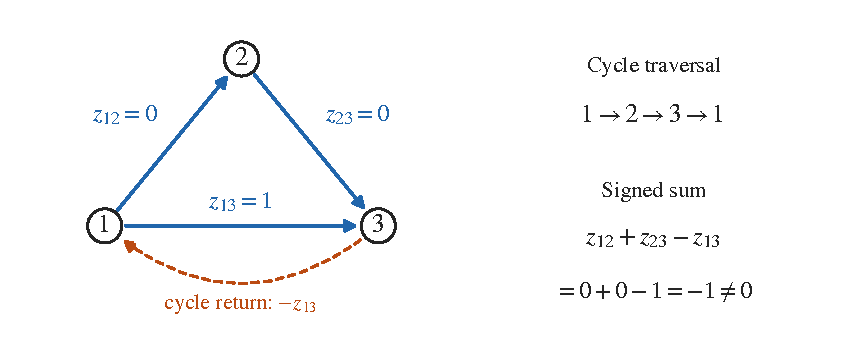
\includegraphics[width=\linewidth]{figures/figure_03_cycle.pdf}
\caption{An abstract observation graph, with no geometric meaning assigned to the vertex positions. Solid arrows orient the three observations in Eq.~\eqref{eq:incompatible-triangle}. The cycle $1\to2\to3\to1$ traverses the $1\to3$ observation backwards (dashed return), giving the contribution $-z_{13}$. This is a signed traversal of the underlying undirected graph, not a fourth observation. Its nonzero sum prevents any single weight vector from reproducing all three targets.}
\label{fig:incompatible-cycle}
\end{figure}
\FloatBarrier

\begin{proposition}[Cycle compatibility]
\label{prop:cycle-compatibility}
Let $G$ be the observation multigraph with incidence matrix $B$ and target differences $z\in\mathbb R^m$. A weight vector $w\in\mathbb R^n$ satisfying $B^Tw=z$ exists if and only if the signed sum of target differences vanishes around every cycle of the underlying undirected multigraph:
\begin{equation}
\sum_{r\in C}\operatorname{sgn}_C(r)\,z_r=0.
\label{eq:cycle-sum}
\end{equation}
Here $\operatorname{sgn}_C(r)=+1$ when the cycle traverses edge $r$ in its assigned orientation and $-1$ otherwise. Cycles formed by two parallel edges are included.
\end{proposition}

\begin{proof}
If $B^Tw=z$, each target difference equals the difference of its endpoint weights. Summing these differences around any cycle gives zero by telescoping.

Conversely, choose a spanning forest of $G$ and assign an arbitrary weight to one root in each connected component. The observations on the forest edges uniquely determine the remaining weights within each component. Every edge outside the forest closes a cycle with the corresponding forest path. By the assumed cycle condition, its target difference agrees with the difference already determined along that path. Thus, all observations are satisfied.
\end{proof}

In particular, repeated observations of the same pair must have identical targets after accounting for their orientations. The construction also leaves one arbitrary additive constant per connected component, leading to the identifiability question considered next.

\begin{corollary}[Identifiability]
\label{cor:observation-identifiability}
Let the observation graph $G$ have $c$ connected components $C_1,\ldots,C_c$, including isolated vertices. If the observations are compatible and $w^\star$ is one solution of $B^Tw=z$, then every solution has the form
\begin{equation}
w=w^\star+\sum_{a=1}^{c}\gamma_a\mathbf{1}_{C_a},
\qquad \gamma_a\in\mathbb R,
\label{eq:component-gauge}
\end{equation}
where $\mathbf{1}_{C_a}$ is the indicator vector of component $C_a$. Consequently, the difference $w_i-w_j$ is uniquely determined by the observations if and only if sites $i$ and $j$ belong to the same connected component. Equivalently, $\operatorname{rank}(B)=n-c$.
\end{corollary}

\begin{proof}
The difference between any two solutions belongs to $\ker B^T$, so it must be constant across every observed edge, and hence within each connected component. Conversely, adding an arbitrary constant to the weights in any component leaves all observed differences unchanged.
\end{proof}

This ambiguity in the observations must be distinguished from a symmetry of the power diagram itself. Adding the same constant to every site weight leaves all power-distance comparisons unchanged and therefore preserves the complete diagram. In contrast, shifting the weights of disconnected observation components independently can change the competition between their cells. Thus, fixing one additive constant per component selects a particular solution, but may also select a particular geometry among several that are equally consistent with the observations.

\subsection{Fitting inconsistent observations}

When the cycle-compatibility conditions of Section~3.1 are violated, no weight vector can satisfy all observations exactly. We therefore seek weights that minimize the discrepancies between the observed separator positions and their predictions under the power model.

For each observation $r$, let $\lambda_r>0$ be the weight assigned to its squared residual in the original measurement units. Using the affine observation model from Section~2, we minimize
\begin{equation}
\mathcal E(w)=\frac12\sum_{r=1}^{m}
\lambda_r\left[
y_r-\beta_r-\alpha_r(w_{i_r}-w_{j_r})
\right]^2.
\label{eq:measured-least-squares}
\end{equation}
With the target differences $z_r=(y_r-\beta_r)/\alpha_r$, the same objective becomes
\begin{equation}
\boxed{
\mathcal E(w)=\frac12\sum_{r=1}^{m}
\rho_r\left[(w_{i_r}-w_{j_r})-z_r\right]^2,
\qquad \rho_r=\lambda_r\alpha_r^2.
}
\label{eq:difference-least-squares}
\end{equation}
This transformation preserves the objective but changes the weights assigned to individual residuals. Since $\alpha_r$ depends on the observation type and connector length, equal weights in the original measurement units do not generally imply equal weights on the inferred differences.

Let $R=\operatorname{diag}(\rho_1,\ldots,\rho_m)$. Using the incidence matrix $B$ from Section~3.1, we can write the objective as
\begin{equation}
\mathcal E(w)=\frac12(B^Tw-z)^TR(B^Tw-z).
\label{eq:matrix-least-squares}
\end{equation}
Differentiation gives
\begin{equation}
\nabla\mathcal E(w)=BR(B^Tw-z).
\end{equation}
Since the objective is convex, its minimizers are characterized by the normal equations
\begin{equation}
\boxed{Lw=BRz,\qquad L=BRB^T.}
\label{eq:laplacian-normal}
\end{equation}

Here $L$ is the weighted graph Laplacian, as in classical graph-potential least squares \cite{Jiang2011}. For any $v\in\mathbb R^n$,
\begin{equation}
v^TLv=\sum_{r=1}^{m}\rho_r(v_{i_r}-v_{j_r})^2\ge 0.
\end{equation}
Since all $\rho_r>0$, this also shows that $\ker L=\ker B^T$, the space of vectors that are constant on each connected component of the observation graph. Moreover, $BRz$ is orthogonal to this nullspace and hence belongs to the range of $L$. Thus, the normal equations have a solution for every $z$, even when the target differences are incompatible. Their solutions differ only by componentwise additive constants. Fixing these unobservable constants selects one representative; we call this a \emph{gauge convention}.

For the inconsistent three-site example in Fig.~\ref{fig:incompatible-cycle}, with equal fitting weights $\rho_r$ and the gauge $w_3=0$, the least-squares solution is
\begin{equation}
(w_1,w_2,w_3)=\left(\frac23,\frac13,0\right).
\end{equation}
The residuals $B^Tw-z=(1/3,\,1/3,\,-1/3)$ follow the order of the three observations. Each therefore has magnitude $1/3$: the fit balances the conflicting observations rather than selecting one to discard.

For fixed generator positions, this quadratic structure also follows from
the interface discrepancy of Spettl et al.\ \cite{Spettl2016}.
For a point $x$ assigned to pair $i,j$, identifying squared generator
radii with the weights gives
\[
\begin{aligned}
z_{ij}(x)
 &=2(p_j-p_i)\cdot x+\|p_i\|^2-\|p_j\|^2,\\
\operatorname{dist}\bigl(x,H_{ij}(w)\bigr)^2
 &=\frac{[(w_i-w_j)-z_{ij}(x)]^2}{4d_{ij}^2}.
\end{aligned}
\]
Summing these terms yields a weighted difference fit of the form above,
up to an overall positive normalization. Multiple points assigned to
one pair can be grouped into their mean target with the corresponding
total fitting weight, plus an additive constant independent of $w$.
This reduction assumes fixed generator positions; the published method
also optimizes those positions.
The additive constant records the spread of the projected sample positions.
Replacing the samples by their mean preserves the optimal weights, but
agreement with that mean need not imply a small error over the sampled
interface. Thus, data sufficient to determine the weights need not suffice
to assess the approximation of an entire boundary.

The quadratic loss is not essential to the observation model. When large residuals should have less influence, the squared penalties can be replaced by convex losses such as the Huber loss, which is quadratic near zero and linear beyond a residual threshold \cite{Huber1964}. The resulting fixed-observation problem remains convex, although its minimizer is generally no longer obtained from a linear Laplacian system.

\subsection{Hard separator constraints}

Some separator requirements must be satisfied exactly rather than treated as approximate targets. We allow a separate set $\mathcal I_{\mathrm H}$ of hard restrictions, which may involve site pairs absent from the $m$ observations used for fitting. For each $h\in\mathcal I_{\mathrm H}$, let $(i_h,j_h)$ be the ordered site pair, and let $[\underline y_h,\overline y_h]$ specify an admissible interval in one of the measurement conventions of Section~2. With the corresponding coefficients $\beta_h$ and $\alpha_h>0$, the restriction reads
\begin{equation}
\underline y_h\le
\beta_h+\alpha_h(w_{i_h}-w_{j_h})
\le\overline y_h.
\label{eq:hard-measurement-interval}
\end{equation}
This is equivalent to the bounds
\begin{equation}
\boxed{\ell_h\le w_{i_h}-w_{j_h}\le u_h,}
\label{eq:hard-weight-interval}
\end{equation}
where
\begin{equation}
\ell_h=\frac{\underline y_h-\beta_h}{\alpha_h},
\qquad
u_h=\frac{\overline y_h-\beta_h}{\alpha_h}.
\end{equation}
An exact separator requirement is the special case $\ell_h=u_h$. Unlike residuals in the least-squares objective, these restrictions must be satisfied by the fitted weights.

Their joint feasibility is described by a directed graph of \emph{difference constraints}: each inequality $w_v\le w_u+c_{uv}$ is represented by an arc $u\to v$ with cost $c_{uv}$. This constraint graph differs from the observation multigraph used for fitting. The standard negative-cycle criterion \cite[Sec.~24.4]{Cormen2009} takes the following form in our sign convention.

\begin{proposition}[Feasibility of difference constraints]
\label{prop:hard-feasibility}
Consider a finite collection of restrictions
\begin{equation}
\ell_h\le w_{i_h}-w_{j_h}\le u_h,
\qquad h\in\mathcal I_{\mathrm H},
\end{equation}
with finite real bounds $\ell_h,u_h$. Construct a directed weighted multigraph on the sites by adding, for each restriction $h$, an arc $j_h\to i_h$ with cost $u_h$ and an arc $i_h\to j_h$ with cost $-\ell_h$.

There exists a weight vector satisfying all restrictions if and only if this graph contains no directed cycle with negative total cost.
\end{proposition}

\begin{proof}
Summing the inequalities represented by arcs around any directed cycle cancels the site weights, so every cycle must have nonnegative total cost.

Conversely, suppose there are no negative directed cycles. Add an auxiliary source connected to every vertex by a zero-cost arc, and let $d(v)$ be the shortest-path distance from this source to vertex $v$. These distances are finite and satisfy
\begin{equation}
d(v)\le d(u)+c_{uv}
\end{equation}
for every arc $u\to v$. Therefore, setting $w_v=d(v)$ satisfies every difference constraint.
\end{proof}

The criterion can be checked using standard shortest-path algorithms, such as Bellman--Ford \cite{Bellman1958}. A negative cycle certifies infeasibility of the prescribed restrictions, independently of any least-squares objective.

When hard restrictions are feasible, they can be imposed on the least-squares fit. Let
\begin{equation}
\mathcal H=\left\{w\in\mathbb R^n:
\ell_h\le w_{i_h}-w_{j_h}\le u_h
\text{ for all }h\in\mathcal I_{\mathrm H}\right\}.
\label{eq:hard-feasible-set}
\end{equation}
The resulting optimization problem is
\begin{equation}
\boxed{
\min_{w\in\mathcal H}
\frac12(B^Tw-z)^TR(B^Tw-z).
}
\label{eq:hard-constrained-fit}
\end{equation}
This is a convex quadratic program. Whenever $\mathcal H$ is nonempty, the minimum is attained, as proved in~\ref{app:constrained-attainment}. Any two minimizers differ by constants on the connected components of the observation graph, but only shifts that preserve $\mathcal H$ remain admissible. In particular, hard restrictions connecting different components may constrain their relative offsets, so independently fixing one constant per component is no longer an arbitrary gauge choice. A common shift of all site weights remains free.

Algebraic compatibility, optimal fitting, and feasibility of hard restrictions do not guarantee that the corresponding site pairs share actual faces in the resulting power diagram. We address geometric realization in the next section.
